%%%%%%%%%%%%%%%%%%%%%%%%%%%%% Define Article %%%%%%%%%%%%%%%%%%%%%%%%%%%%%%%%%%
\documentclass{article}
%%%%%%%%%%%%%%%%%%%%%%%%%%%%%%%%%%%%%%%%%%%%%%%%%%%%%%%%%%%%%%%%%%%%%%%%%%%%%%%

%%%%%%%%%%%%%%%%%%%%%%%%%%%%% Using Packages %%%%%%%%%%%%%%%%%%%%%%%%%%%%%%%%%%
\usepackage{listings, xcolor}
\usepackage{parskip}
\usepackage{hyperref}
\usepackage{amsmath}
\usepackage{graphicx}
\usepackage[a4paper, margin = 1.5cm]{geometry}
\usepackage{float}
\usepackage{amsmath}
\usepackage{amssymb}
\usepackage{parskip}
\usepackage{listings}
\usepackage{physics}

\lstset{
frame = shadowbox,
basicstyle = \small\ttfamily,
mathescape = true,
numbers = left,
commentstyle = \itshape\color{gray}
columns = flexible,
keepspaces = true,
moredelim = [l]{//}
}

%%%%%%%%%%%%%%%%%%%%%%%%%%%%%% Title & Author %%%%%%%%%%%%%%%%%%%%%%%%%%%%%%%%
\title{Riassunto Social Computing}
\author{Trentin Tommaso}
%%%%%%%%%%%%%%%%%%%%%%%%%%%%%%%%%%%%%%%%%%%%%%%%%%%%%%%%%%%%%%%%%%%%%%%%%%%%%%
\begin{document}
\maketitle
\tableofcontents
\newpage

\section{Social media}
  Tecnologie che facilitano \textbf{creazione} e \textbf{condivisione} di informazioni, idee, interessi e altre forme di espressione mediante \textbf{community vistuali} e \textbf{network}.
  \begin{itemize}
      \item Applicazioni internet-based \textbf{Web 2.0};
      \item Sviluppate avendo come scopo principale la gestione di \textbf{User-generated content};
      \item Utenti creano \textbf{profili} e identità service-specific che vengono mantenuti dalla social media organization;
      \item Facilitano lo sviluppo di \textbf{social network online} connettendo il profilo di un utente con quello di altri individui / organizzazioni.
  \end{itemize}

  \subsection{Classificazione}
    2 dimensioni principali: \textbf{Social presence / Media richness} (quanto sembra di essere "lì") e \textbf{Self presentation / Self disclosure} (quanto si rivela di sé).
    \begin{figure}[H]
        \centering
        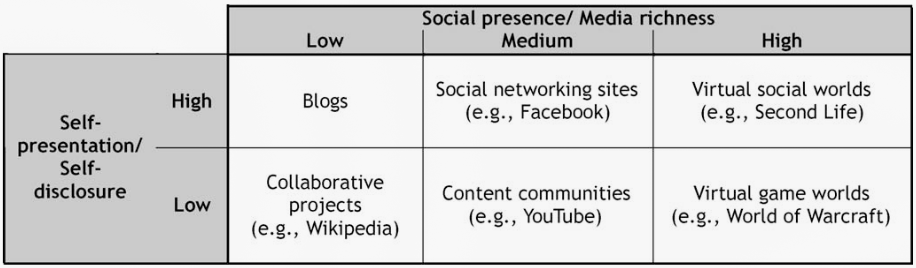
\includegraphics[width=0.6\linewidth]{figures/sm_cla.png}
    \end{figure}
    Visione articolata:
    \begin{figure}[H]
        \centering
        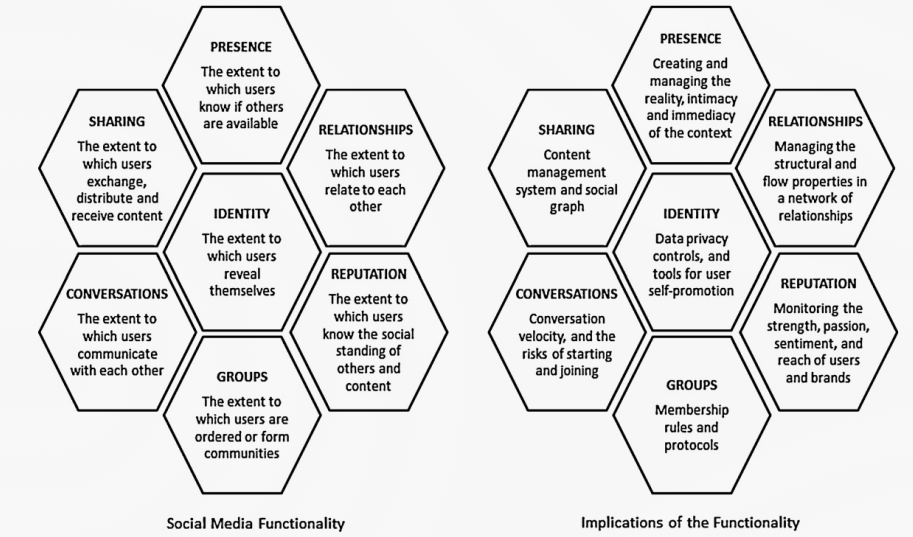
\includegraphics[width=0.5\linewidth]{figures/sm_cla_alt.png}
    \end{figure}

\section{Grafi e Reti}
  \subsection{Nodi vs. Attori (dipende dal contesto)}
    $$V={v_1,v_2,...,v_n}$$
    \begin{itemize}
        \item Grafo del Web:
           \begin{itemize}
               \item Nodi = pagine/siti web;
               \item Archi = link ipertestuali.
           \end{itemize}
        \item Grafo sociale di amicizie:
          \begin{itemize}
               \item Nodi = persone;
               \item Archi = amicizie, conoscenze...
          \end{itemize}
    \end{itemize}
    \textbf{Grandezza del grafo} (size): $\abs{V}=n$
  \subsection{Archi}
    $$E={e_1,e_2,...,e_m}$$
    Gli archi (edges) connettono nodi (ties / relationships). In un settng sociale:
    \begin{itemize}
        \item Nodi = entità sociali (persone);
        \item Archi = relazioni fra persone;
    \end{itemize}
    \textbf{Grandezza dell'insieme degli archi}: $\abs{E}=m$
  \subsection{Grafi}
    Un grafo \textit{G} si può rappresentare come coppia dell'insieme di nodi \textit{V} e archi \textit{E}:
    $$G(V,E)$$
    \subsubsection{Proprietà}
      \begin{itemize}
          \item Archi possono avere direzioni ($e(v_1,v_2) \neq e(v_2,v_1)$);
          \item \textbf{Grafo pesato}: ad ogni arco è associato un peso ($G(V,E,W)$);
          \item Grafo $G'(V',E')$ è \textbf{sottografo} di $G(V,E)$ se ($V' \subseteq V$) e ($E' \subseteq (V' \times V') \cap E$);
          \item \textbf{Vicinato} di un nodo: tutti i nodi ad esso collegati mediante archi (incoming / outgoing neighbors);
          \item \textbf{Cammino}: sequenza di archi t.c. ogni arco è incidente allo stesso nodo del successivo;
          \item \textbf{Connessione}:
            \begin{itemize}
                \item Un \textbf{nodo} $v_i$ è connesso al nodo $v_j$ se esiste cammino da $v_i$ a $v_j$ (e viceversa);
                \item Un \textbf{grafo} è connesso se esiste un cammino fra ogni coppia di nodi (\textit{fortemente} se il cammino è diretto, \textit{debolmente} altrimenti)
            \end{itemize}
          \item \textbf{Componenti}:
            \begin{itemize}
                \item \textbf{Componente in un grafo indiretto}: è un sottografo massimale connesso.
                \begin{itemize}
                    \item Esiste un cammino indiretto fra ogni coppia di nodi nella componente.
                    \item \textit{"Massimale"} significa che se si aggiungono altri nodi del grafo originale, il sottografo non è più connesso.
                \end{itemize}
                \item \textbf{Componente Fortemente Connessa} (Strongly Connected Component, \textbf{SCC}): In un grafo diretto, si ha una SCC quando per ogni coppia di nodi $u, v \in \text{SCC}$ esiste un cammino \textit{diretto} da $u$ a $v$ e uno da $v$ a $u$.
                \item \textbf{Componente Debolmente Connessa} (Weakly Connected Component, \textbf{WCC}): In un grafo diretto, si ha una WCC quando per ogni coppia di nodi $u, v \in \text{WCC}$ esiste un cammino \textit{indiretto} da $u$ a $v$.
                \item Un grafo può avere diverse componenti (ne ha solo 1 se l'intero grafo è connesso).
                \item \textbf{Giant Connected Component}: è la componente più grande del grafo e contiene "quasi tutto" il grafo (la maggior parte dei nodi).
            \end{itemize} 
      \end{itemize}
  \subsection{Gradi}
    $\pi(d)={d_1,d_2,...,d_n}$
    \textbf{Grado di un nodo $i$} $d_i$: numero di archi collegati a quel nodo (entranti = \textbf{in-degree} $d^{in}_i$, uscenti = \textbf{out-degree} $d^{out}_i$).
    \\
    \textbf{Degree distribution}: per ogni nodo, quanti nodi hanno quel grado:
    $$p_{grado}=\frac{numNodi_grado}{numNodi}, \sum_{d=0}^{\inf}p_{grado}=1$$
    \\
    \textbf{Teorema}: sommatoria dei gradi di un grafo indiretto è 2 volte il numero degli archi
    $$\sum_id_i=2\abs{E}$$
    \textbf{Corollari}:
    \begin{enumerate}
        \item numero di nodi con grado dispari è pari;
        \item in ogni grafo diretto la sommatoria degli in-degree è uguale alla somma degli out-degree
    \end{enumerate}
    $$\sum_id^{out}_i=\sum_jd^{in}_j$$
    \begin{figure}[H]
        \centering
        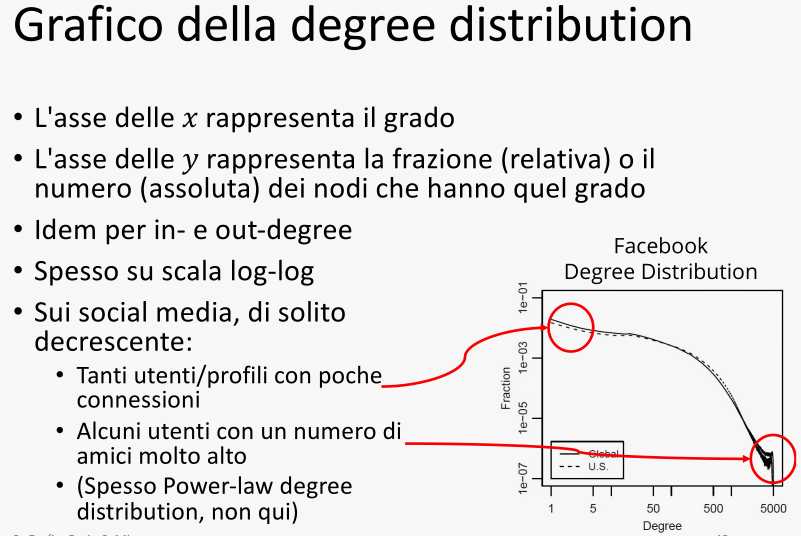
\includegraphics[width=0.5\linewidth]{figures/deg_distr.png}
    \end{figure}
  \subsection{Densità}
    Quanti archi ci sono rispetto a tutti gli archi possibili:
    \begin{itemize}
      \item Grafi \textbf{indiretti} - $D=\frac{2\abs{E}}{\abs{V}(\abs{V}-1)}$
      \item Grafi \textbf{diretti} - $D=\frac{\abs{E}}{\abs{V}(\abs{V}-1)}$
    \end{itemize}
  \subsection{Rappresentazioni}
    \subsubsection{Lista degli archi}
      \begin{itemize}
          \item Ogni elemento della lista è un arco da un nodo u a un nodo v $(u,v)$;
          \item Ok anche per grafi diretti; 
          \item Non ok per nodi isolati: non vengono rappresentati.
      \end{itemize}
      \begin{figure}[H]
          \centering
          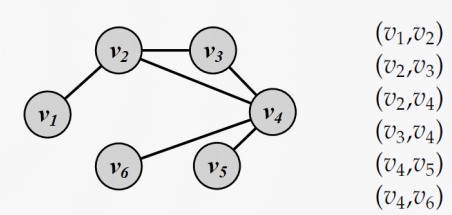
\includegraphics[width=0.5\linewidth]{figures/l_ar.png}
      \end{figure}
    \subsubsection{Lista di adiacenza}
      \begin{itemize}
          \item Per ogni nodo, lista di tutti i nodi a cui è connesso;
          \item Solitamente ordinata;
          \item Ok anche per grafi diretti.
      \end{itemize}
      \begin{figure}[H]
          \centering
          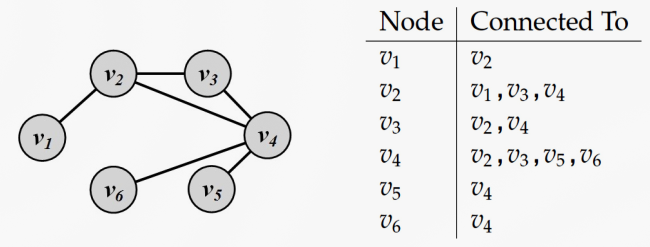
\includegraphics[width=0.5\linewidth]{figures/l_ad.png}
      \end{figure}
    \subsubsection{Matrice di adiacenza}
      \begin{itemize}
          \item Quadrata (1 se c'è un arco fra $v_i$ e $v_j$, 0 altrimenti);
          \item Simmetrica per grafi indiretti;
          \item Ok per grafi diretti (generalmente non simmetrica);
          \item Auto-archi (self-link) sulla diagonale;
          \item Per reti sociali le matrici di adiacenza sono sparse (quasi tutti 0);
          \item Ok per grafi pesati ()
          \item Quadrata ($w_{ij}$ se c'è un arco fra $v_i$ e $v_j$, 0 altrimenti);
      \end{itemize}
      \begin{figure}[H]
          \centering
          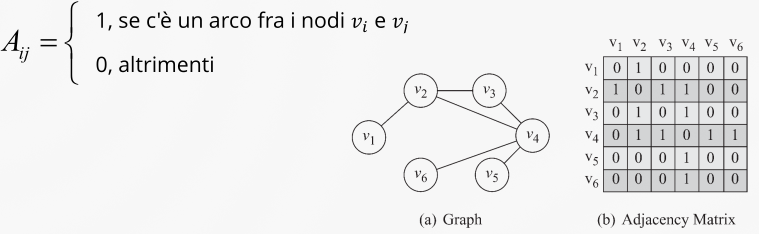
\includegraphics[width=0.5\linewidth]{figures/mat_ad.png}
      \end{figure}
  \subsection{Reti}
    Una rete (\textbf{network}) è un grafo (solitamente grande) con nodi e archi che esistono nel mondo reale, solitamente per rappresentare problemi su una rete si usano grafi e risultati della teoria dei grafi.
    \subsubsection{Reti sociali}
      Reti i cui elementi hanno una struttura sociale:
      \begin{itemize}
          \item Insieme di \textbf{attori} = individui / organizzazioni;
          \item Insieme di \textbf{legami} = connessioni fra attori.
      \end{itemize}
      Esempi: rete di familiari / amici / colleghi.
    \subsubsection{Analisi delle reti sociali (Social Network Analysis - SNA)}
      Settore interdisciplinare (scienze sociali + statistica + teoria dei grafi + reti complesse + informatica) che studia queste reti.
\section{Reti e Misure}
  \subsection{Centralià}
    \textbf{Misura} che indica quanto un nodo è centrale, basandosi su definizioni / assunzioni.
    \subsubsection{Centralità di grado}
      Più è alto il grado di un nodo, più è centrale.
      $$C_d(v_i)=d_i$$
      \begin{figure}[H]
          \centering
          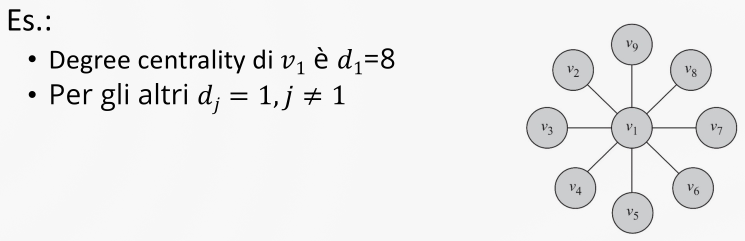
\includegraphics[width=0.6\linewidth]{figures/deg_cen.png}
      \end{figure}
      In grafi diretti si possono usare in-degree, out-degree o combinazione dei due:
      \begin{itemize}
        \item $C_d(v_i)=d^{in}_i$ (prestige);
        \item $C_d(v_i)=d^{out}_i$ (gregariousness);
        \item $C_d(v_i)=d^{in}_i+d^{out}_i$.
      \end{itemize}
      In pratica in-degree è il più usato / interessante.
    \subsubsection{Centralità di grado normalizzata}
      Utile per confrontare grafi differenti:
      \begin{itemize}
        \item Normalizzazione per grado massimo possibile - $C^{norm}_d(v_i)=\frac{d_i}{n-1}$;
        \item Normalizzazione per grado massimo effettivo - $C^{max}_d(v_i)=\frac{d_i}{max_jd_j}$;
        \item Normalizzazione per somma dei gradi - $C^{sum}_d(v_i)=\frac{d_i}{\sum_jd_j}=\frac{d_i}{2\abs{E}}=\frac{d_i}{2m}$.
      \end{itemize}
      \begin{figure}[H]
          \centering
          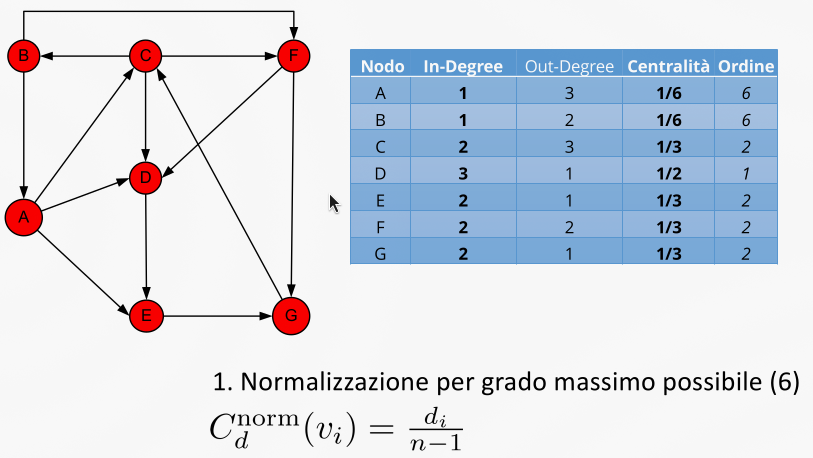
\includegraphics[width=0.5\linewidth]{figures/deg_cen_n.png}
      \end{figure}
    \subsubsection{Betweenness centrality}
      Misura quanto un nodo è importante nel connettere altri nodi tramite cammini (si guradano solo shortest paths).
      $$C_b(v_i)=\sum_{s\neq t\neq v_i}\frac{\sigma_{st}(v_i)}{\sigma_{st}}$$
      \begin{itemize}
        \item $\sigma_{st}(v_i)$: numero di shortest paths da $s$ a $t$ che passano per $v_i$;
        \item $\sigma_{st}$: nuemero di shortest paths da $s$ a $t$.
      \end{itemize}
      \begin{figure}[H]
          \centering
          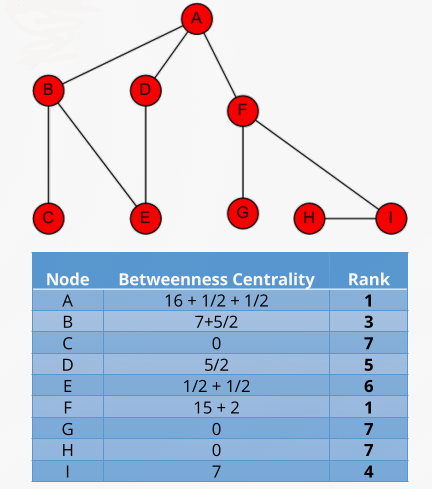
\includegraphics[width=0.4\linewidth]{figures/bet_cen.png}
      \end{figure}
    \subsubsection{Betweenness centrality normalizzata}
      Nel caso migliore il nodo $v_i$ è su tutti gli shortest paths da $s$ a $t$, quindi $\frac{\sigma_{st}(v_i)}{\sigma_{st}}=1,\forall s,t$
      $$C_b(v_i)=\sum_{s\neq t\neq v_i}\frac{\sigma_{st}(v_i)}{\sigma_{st}}=\sum_{s\neq t\neq v_i}1=2\binom{n-1}{2} = (n-1)(n-2)$$
      Quindi il valore massimo è $(n-1)(n-2)$, per normalizzarlo:
      $C^{norm}_b(v_i)=\frac{C_b(v_i)}{2(\binom{n-1}{2})}$
    \subsubsection{Centralità di vicinanza (Closeness centrality)}
      $$C_c(v_i)=\frac{1}{\bar{l}_{v_i}}$$
      I nodi influenti / centrali possono raggiungere velocemente gli altri nodi (considero gli shortest path verso tutti gli altri nodi).
      $$\bar{l}_{v_i}=\frac{1}{n-1}\sum_{v_j\neq v_i}l_{i,j}$$
      \begin{itemize}
        \item $l_{i,j}$: lunghezza cammino più breve da $v_i$ a $v_j$;
        \item $\bar{l}_{v_i}$: lunghezza media dei cammini più brevi più brevi da $v_i$.
      \end{itemize}
      \begin{figure}[H]
          \centering
          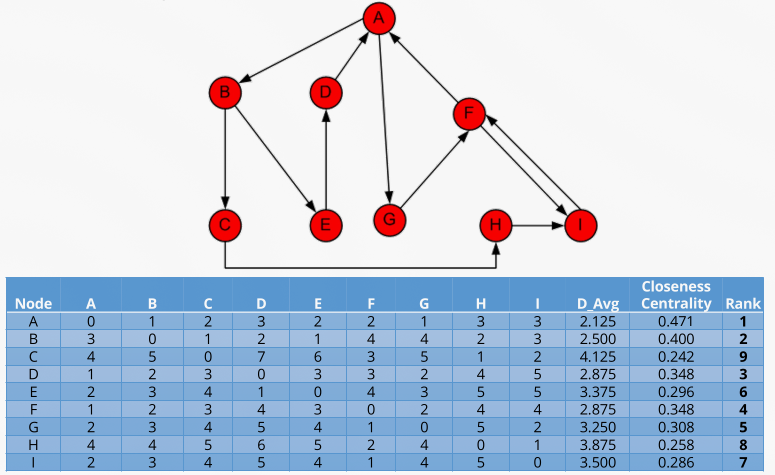
\includegraphics[width=0.5\linewidth]{figures/cl_cen.png}
      \end{figure}
    \subsubsection{Confronti}
      \begin{figure}[H]
          \centering
          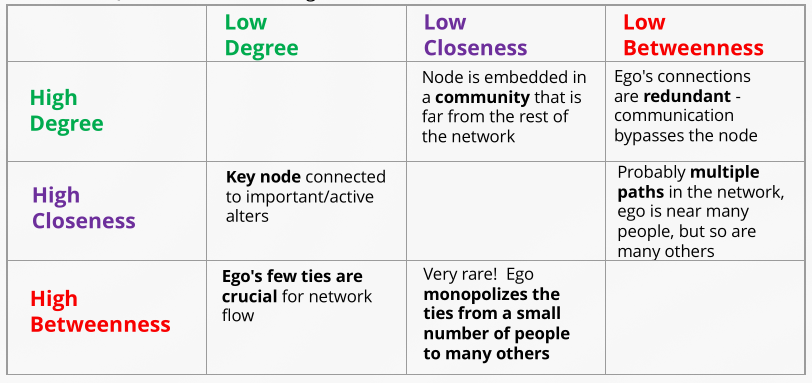
\includegraphics[width=0.6\linewidth]{figures/centr_chart.png}
      \end{figure}
  \subsection{PageRank}
    Archi che vengono da \textbf{nodi importanti} (più centrali) dovrebbero \textbf{aumentare di più la centralità} rispetto a archi che vengono da nodi meno centrali.
    \begin{figure}[H]
        \centering
        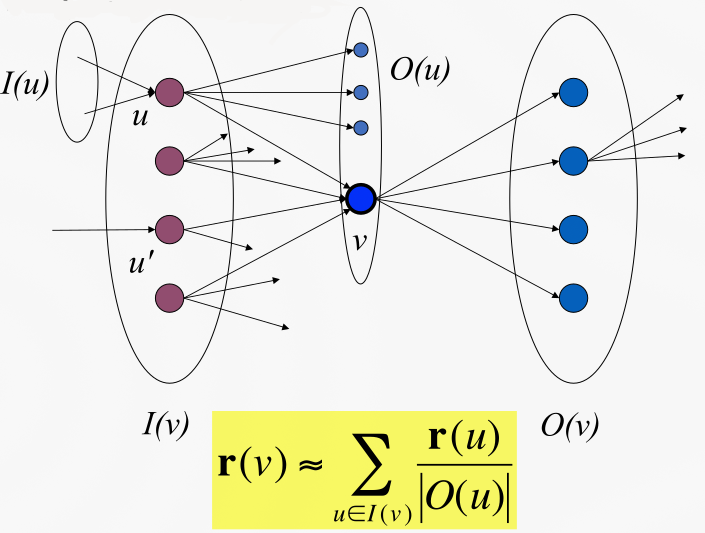
\includegraphics[width=0.3\linewidth]{figures/p_rank.png}
    \end{figure}
    Notazione:
    \begin{itemize}
        \item $r(v)$ PageRank della pagina $v$;
        \item $I(v)$ set di paine che citano $v$;
        \item $O(v)$ set di pagine citate da $v$.
    \end{itemize}
    Ogni pagina $u$ ha il suo valore PageRank $r(u)$, la pagina $v$ riceve dalla pagina $u$ una porzione del suo PageRank uguale alla porzione ricevuta da tutte le altre pagine citate da $u$: $\frac{r(u)}{\abs{O(u)}}$
    \subsubsection{PageRank - vettori e matrici}
      Si possono collezionare tutti i valori PageRank di tutte le pagine $u_i$ in un vettore $r=[r(u_0), r(u_1), ..., r(u_n)$ 
      \\
      \noindent
        \begin{minipage}[t]{0.48\linewidth}
          Si costruiscono i vettori $r$ \textbf{iterativamente, tutti assieme}. Per andare da $r_0$ iniziale a $r_1$ mediante una matrice \textbf{P} tale che $r_{i+1}=r_i\times P$
        \end{minipage}
        \hfill
        \begin{minipage}[c]{0.48\linewidth}
            \centering
            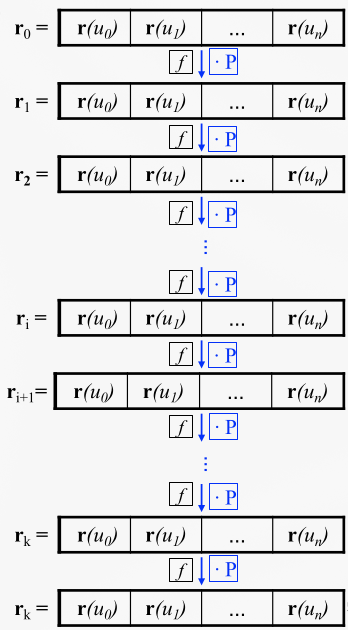
\includegraphics[width=0.5\linewidth]{figures/p_rank_m.png}
        \end{minipage}
    \subsubsection{Markov chain}
      Dato un grafo / matrice di adiacenza con $n$ stati si ha una matrice $n\times n$ P con le probabilità di transizione. A ciascun istante di tempo la catena di Markov è in uno degli $n$ stati.
      \\
      $\forall$ stato corrente $i\in [1..n]$, la catena di Markov (\textbf{P}) dice la probabilità che il prossimo stato sia $j$, $\forall j\in [1..n]$.
      \begin{figure}[H]
          \centering
          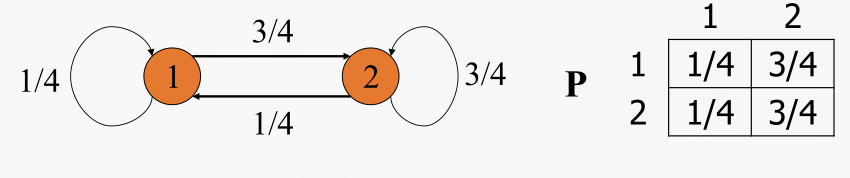
\includegraphics[width=0.7\linewidth]{figures/mar_ch.png}
      \end{figure}
      Si può rappresentare la posizione corrente in uno stato $i$ con un vettore $x=(x_1,...,x_n)$ dove tutti i componenti hanno valore 0 tranne l'$i$-esimo che ha valore 1 e rappresenta la posizione nello stato $i$.
      \\
      Il vettore di probabilità nel prossimo step si può trovare guardando la matrice P alla $i$-esima riga, in modo da controllare le probabilità per procedere al prossimo stato partendo da $i$.
    \subsubsection{Markov chain - autovettore}
      Quindi, per ogni step $x_{i+1}=x_i\times P$ ma stiamo cercando una distribuzione stabile $x_{i+1}=x_i$, cerchiamo quindi $x$ tale che $x=x\times P$ ($x$ autovettore di $P$).
      \\
      Per ogni catena \textbf{ergodica} (\textbf{fortemente connessa} e in cui in ogni step si può \textbf{essere in ogni stato} con probabilità > 0) ogni stato ha un rate di visite a lungo termine per cui viene visitato proporzionalmente.
    \subsubsection{Teleporting}
      Nella pratica (Web) non sempre si hanno situazioni ergodiche, ma navigando si potrebbe "saltare" ad un'altra pagina random: "ciascuna pagina è collegata con qualsiasi altra pagina" (con basse probabilità).
      \begin{figure}[H]
          \centering
          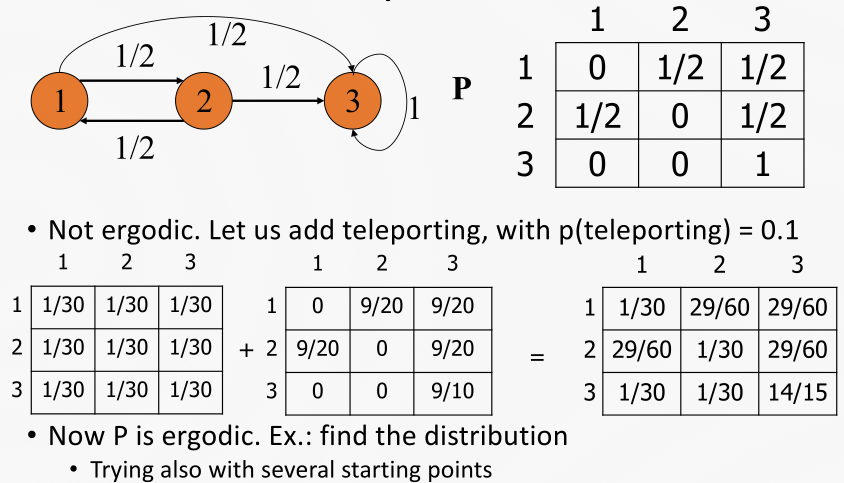
\includegraphics[width=0.6\linewidth]{figures/telep.png}
      \end{figure}
    \subsubsection{PageRank - implementazione}
      Catena di Markov, ogni pagina ha una propria probabilità per cui, durante il percorso random tra le pagine, l'utente si trovi lì
      \begin{figure}[H]
          \centering
          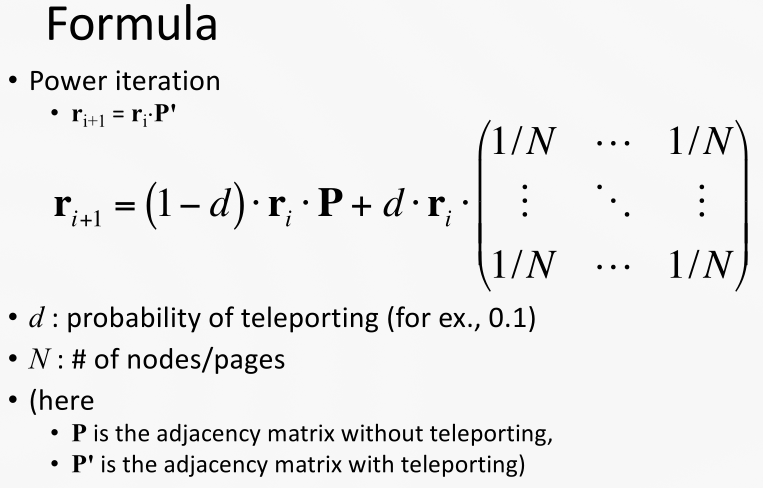
\includegraphics[width=0.4\linewidth]{figures/pr_impl.png}
      \end{figure}
      \begin{enumerate}
          \item Costruzione matrice $P'$ (matrice di adiacenza $P$ + teleporting (ergodic));
          \item Inizio da vettore di probabilità $r_0$;
          \item $r_{i+1}=r_i\times P$;
          \item Se $\abs{r_{i+1}-r_i} < \epsilon$ stoppa, altrimenti ripeti;
          \item Il vettore $r$ trovato ($r=r\times P'$, o $r~r\times P'$) è il PageRank di tutte le pagine, e ~ l'autovettore di $P'$.
      \end{enumerate}
  \subsection{HITS}
    Idea: costruire 2 set di pagine collegati:
    \begin{itemize}
        \item \textbf{Hub pages (H)} contenenti (buoni) link ad altre pagine (yahoo, buoni bookmark,...);
        \item \textbf{Authority pages (A)} con persone / entità ben organizzate nel web (w3c, Knuth's homepage,...).
    \end{itemize}
\end{document}
